\documentclass[12pt]{exam}
\usepackage[utf8]{inputenc}
\usepackage[T1]{fontenc}

\usepackage{amsmath}
\usepackage{amssymb}

\usepackage[a4paper, total={6.5in, 10in}]{geometry}
\usepackage[ngerman]{babel}
\usepackage{pdfpages}
\usepackage{graphicx}
\usepackage{xcolor}
\usepackage{siunitx}
\usepackage{minted}
\usepackage{hyperref}

\newcommand{\del}{\partial}

\footer{}{\thepage}{}

\begin{document}

\begingroup  
    \centering
    \Large Proseminar Modellierung\\
    \Large Blatt 3\\[0.75em]
    \large \today\\[0.75em]
    \normalsize Andreas Mair, Christina Schwaiger, Martin Fuchs \& Morris-Luca Kühmeier\par
\endgroup

\vspace{12pt}
\hrule
\vspace{12pt}

\printanswers
\renewcommand{\solutiontitle}{\textbf{Lösung:}\enspace}

\thispagestyle{plain}

\begin{questions}

    \question Explain why it is physically reasonable to impose the boundary condition $n \cdot u = 0$ for a solid object immersed in a fluid.
    
    \begin{solution}
        Die Stromlinien unweit des Randes eines in einer Flüssigkeiten untergetauchten Objektes verlaufen nahezu tangential zu dessen Oberfläche, da diese für die Flüssigkeit undurchlässig ist. Die Richtung des Geschwindigkeitsfeldes steht also an der Oberfläche orthogonal auf das Einheitsnormalenfeld.

        \centering
        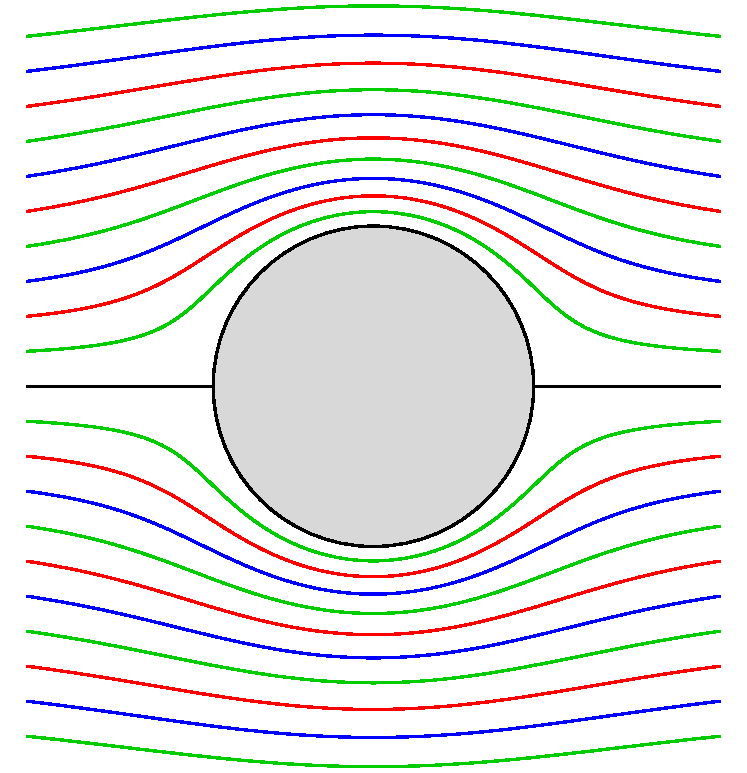
\includegraphics[width=0.5\textwidth]{LaminarFlow.pdf}\\
        Die Stromlinien am Beispiel eines Zylinders
    \end{solution}
    
    
    \question Imagine a (small) fluid element of velocity $(u_1, v_1)$, pressure $p_1$, volume $V_1$, and density $\rho_1$. The energy stored in that fluid element is
    \begin{equation*}
        E_1 = V_1 \left( p_1 + \frac{1}{2} \rho_1 (u^2_1 + v^2_1) \right).
    \end{equation*}
    Show that $E_1$ is indeed measured in units of energy. \newline
    Now, our fluid elements moves with the fluid and at a later time it has velocity $(u_2, v_2)$, pressure $p_2$, and volume $V_2$. Show that we can derive Bernoulli's equation
    \begin{equation*}
        p_1 + \frac{1}{2} \rho (u^2_1 + v^2_1) = p_2 + \frac{1}{2} \rho (u^2_2 + v^2_2)
    \end{equation*}
    by assuming conservation of energy, i.e. $E_1 = E_2$, and an incompressible fluid, i.e. $V_1 = V_2$ and $\rho := \rho_1 = \rho_2$
    
    \begin{solution}
        Die Einheit von $E_1$ berechnet sich zu
        \begin{equation*}
            \left[ E_1 \right] = \left[ V_1 \left( p_1 + \frac{1}{2} \rho_1 (u^2_1 + v^2_1) \right) \right] = \left[ V_1 \right] \left[ \rho_1 \right] \left[ u_1 \right]^2 = \mathsf{L}^3 \, \mathsf{M} \, \mathsf{L}^{-3} \, \mathsf{L}^2 \, \mathsf{T}^{-2} = \mathsf{M} \, \mathsf{L}^2 \, \mathsf{T}^{-2},
        \end{equation*}
        was gerade die Einheit der Energie ist. Ist nun
        \begin{equation*}
            E_1 = V_1 \left( p_1 + \frac{1}{2} \rho_1 (u^2_1 + v^2_1) \right)
            \quad \text{und} \quad
            E_2 = V_2 \left( p_2 + \frac{1}{2} \rho_2 (u^2_2 + v^2_2) \right),
        \end{equation*}
        ergibt sich dann unter Annahme, dass $E_1 = E_2$, $V_1 = V_2$ und $\rho := \rho_1 = \rho_2$ sofort
        \begin{equation*}
            V_1 \left( p_1 + \frac{1}{2} \rho (u^2_1 + v^2_1) \right) = V_1 \left( p_2 + \frac{1}{2} \rho (u^2_2 + v^2_2) \right).
        \end{equation*}
        Division durch $V_1$ zeigt die gewünschte Gleichheit
        \begin{equation*}
            p_1 + \frac{1}{2} \rho (u^2_1 + v^2_1) = p_2 + \frac{1}{2} \rho (u^2_2 + v^2_2).
        \end{equation*}
    \end{solution}
    
    
    \question Show that a streamfunction $\psi$, i.e. $u = \del_y \psi$ and $v = -\del_x \psi$, satisfies the incompressibility condition. That is, $\nabla \cdot u = 0$. Then show that
    \begin{equation*}
        \Delta \phi = 0 \iff \Delta \psi = 0.
    \end{equation*}
    
    \begin{solution}
        Unter der Annahme, dass die Stromfunktion zwei mal partiell differenzierbar ist, folgt
        \begin{equation*}
            \nabla \cdot u = \frac{\del u}{\del x} + \frac{\del v}{\del y} = \frac{\del^2 \psi}{\del x \del y} - \frac{\del^2 \psi}{\del y \del x} = 0.
        \end{equation*}
        Wenden wir uns der zweiten Aussage zu. Es ist $\varphi + i \psi$ als Stammfunktion einer analytischen Funktion analytisch, sodass Real- und Imaginärteil harmonisch sind, d.h. $\Delta \varphi = \Delta \psi = 0$.
    \end{solution}
    
    
    \question Calculate the potential for the uniform flow over a cylinder. What units are associated with the streamfunction and the potential?
    
    \begin{solution}
        Da $x = r \cos \theta$ und $y = r \sin \theta$, erfüllen $\phi$ und $\psi$
        \begin{equation*}
            \frac{\del \phi}{\del r} = \frac{1}{r} \frac{\del \psi}{ \del \theta} \quad \text{und} \quad \frac{1}{r} \frac{\del \phi}{\del \theta} = -\frac{\del \psi}{\del r}.
        \end{equation*}
        Aus der Vorlesung kennen wir $\psi$ (Herleitung siehe unten) als
        \begin{equation*}
            \psi = V_{\infty} r \sin \theta \left( 1 - \frac{R^2}{r^2} \right).
        \end{equation*}
        Ableiten nach $\theta$ und $r$ ergibt
        \begin{align*}
            \frac{1}{r} \frac{\del \psi}{\del \theta} &=  V_{\infty} \cos \theta \left( 1 - \frac{R^2}{r^2} \right) \\
            -r \frac{\del \psi}{\del r} &= -V_{\infty} r \sin \theta \left( 1 + \frac{R^2}{r^2} \right).
        \end{align*}
        Integration nach $\theta$ respektive $r$ führt auf
        \begin{equation*}
            \phi = V_{\infty} r \cos \theta \left( 1 + \frac{R^2}{r^2} \right).
        \end{equation*}
        Wir führen noch eine Dimensionsanalyse für $\phi$ und $\psi$ durch. Es gilt
        \begin{equation*}
            \frac{[\del \psi]}{[\del y]} = \frac{[\del \phi]}{[\del x]} = [u] = \mathsf{L} \, \mathsf{T}^{-1}.
        \end{equation*}
        Dabei ist $[\del x] = [\del y] = \mathsf{L}$, also
        \begin{equation*}
            [\psi] = [\phi] = \mathsf{L}^2 \, \mathsf{T}^{-1}.
        \end{equation*}
        
        \textbf{Herleitung:} \\
        Der Laplace-Operator schreibt sich für bekanntlich in Polarkoordinaten als
        \begin{equation*}
            \frac{1}{r} \frac{\del}{\del r} \left( r \frac{\del \psi}{\del r} \right) + \frac{1}{r^2} \frac{\del^2 \psi}{\del \theta^2}.
        \end{equation*}
        Wir verfolgen einen Separationsansatz zur Lösung der Laplace-Gleichung und schreiben
        \begin{equation*}
            \psi(r, \theta) = R(r) \Theta(\theta).
        \end{equation*}
        Einsetzen führt dann zu
        \begin{align*}
            \frac{1}{r} \frac{\del}{\del r} \left( r \Theta(\theta) R'(r) \right) + \frac{1}{r^2} R(r) \Theta''(\theta) &= 0 \\
            \frac{1}{r} \left( \Theta(\theta) R'(r) + r \Theta(\theta) R''(r) \right) + \frac{1}{r^2} R(r) \Theta''(\theta) &= 0 \\
            \frac{r R'(r) + r^2 R''(r)}{R(r)} &= -\frac{\Theta''(\theta)}{\Theta(\theta)} = \lambda^2.
        \end{align*}
        Lösen dieser beiden Differentialgleichungen ergibt
        \begin{align*}
            \Theta(\theta) &= A \cos(\lambda \theta) + B \sin(\lambda \theta) \\
            R(r) &= a r^{\lambda} + b r^{-\lambda}.
        \end{align*}
        Fordern wir die Stetigkeit von $\psi$ in $\theta$, d.h. $\psi(r, \theta) = \psi(r, \theta + 2 n \pi)$, dann muss $\lambda \in \mathbb{N}$ sein. Somit schreibt sich die Lösung als
        \begin{equation*}
            \psi(r, \theta) = \sum_{n=1}^{\infty} (a_n r^n + b_n r^{-n})(A_n \cos(n \theta) + B_n \sin(n \theta)).
        \end{equation*}
        Nun gilt es die Randbedingungen zu erfüllen, denn es sollen
        \begin{equation*}
            \frac{\del \psi}{\del \theta} \bigg\vert_{r=R} = 0
        \end{equation*}
        und
        \begin{equation*}
            \psi = V_{\infty} r \sin \theta \quad \text{für} \quad r = \infty
        \end{equation*}
        gelten, wobei $R$ den Radius des Zylinders beschreibt. Betrachten wir zuerst
        \begin{equation*}
            \lim_{r \to \infty} V_{\infty} r \sin(\theta) \overset{!}{=} \lim_{r \to \infty} \sum_{n=1}^{\infty} (a_n r^n + b_n r^{-n})(A_n \cos(n \theta) + B_n \sin(n \theta)).
        \end{equation*}
        Daran sehen wir nun per Vergleich der Koeffizienten, dass
        \begin{equation*}
            a_1 B_1 = V_{\infty}, \quad A_1 = 0  \quad \text{und} \quad a_n = b_n = A_n = B_n = 0 \quad \text{für} \; n \geq 2
        \end{equation*}
        Zusammengefasst ergibt sich also
        \begin{equation*}
            \psi = V_{\infty} \left( r + \frac{b_1}{a_1} \frac{1}{r} \right) \sin \theta.
        \end{equation*}
        Im letzten Schritt ist noch eine weitere Randbedingung unterzubringen. Zu diesem Zweck leiten wir nach $\theta$ ab, setzen $r = R$ und erhalten
        \begin{equation*}
            - V_{\infty} \left( R + \frac{b_1}{a_1} \frac{1}{R} \right) \cos \theta \overset{!}{=} 0
        \end{equation*}
        Offensichtlich gilt das im Falle $\frac{b_1}{a_1} = -R^2$. Das führt dann aber auf die gesuchte Lösung
        \begin{equation*}
            \psi = V_{\infty} r \sin \theta - \frac{\kappa}{2 \pi} \frac{\sin \theta}{r}
        \end{equation*}
        mit $\kappa = 2 \pi V_{\infty} R^2$.
    \end{solution}
    
    
    \question The Euler equation of gas dynamics can be written as
    \begin{align*}
        \del_t \rho + (\rho v_1)_x + (\rho v_2)_y + (\rho v_3)_z &= 0 \\
        \del_t V + F(V)_x + G(V)_y + H(V)_z &= 0 \\
        \del_t E + ((E + p)v_1)_x + ((E + p)v_2)_y + ((E + p)v_3)_z &= 0 \\
        E &= \rho \left( \frac{v^2}{2} + \frac{p}{(1-\gamma) \rho} \right)
    \end{align*}
    with
    \begin{equation*}
        V = 
        \begin{bmatrix}
            \rho v_1 \\
            \rho v_2 \\
            \rho v_3
        \end{bmatrix}, \quad
        F(V) =
        \begin{bmatrix}
            \rho v_1^2 + p \\
            \rho v_1 v_2 \\
            \rho v_1 v_3
        \end{bmatrix}, \quad
        G(V) =
        \begin{bmatrix}
            \rho v_1 v_2 \\
            \rho v_2^2 \\
            \rho v_2 v_3
        \end{bmatrix}, \quad
        H(V) =
        \begin{bmatrix}
            \rho v_1 v_3 \\
            \rho v_2 v_3 \\
            \rho v_3^2 + p
        \end{bmatrix}.
    \end{equation*}
    Perform a non-dimensionalization of this equation. \newline
    Hint: Choose a characteristics length scale $L$, characteristic velocity $V_{\infty}$, and characteristic density $\rho_{\infty}$ and then proceed as we did in the lecture.
    
    \begin{solution}
        Wir setzen
        \begin{equation*}
            X = \frac{x}{L}, \quad V = \frac{v}{V_{\infty}}, \quad D = \frac{\rho}{\rho_{\infty}}, \quad P = \frac{p}{\rho_{\infty} V_{\infty}^2}, \quad T = \frac{t}{L/V_{\infty}} \quad \text{und} \quad \widehat{E} = \frac{E}{\rho_{\infty} V_{\infty}^2 L^3} 
        \end{equation*}
        Für die erste Gleichung führt das auf
        \begin{align*}
            \rho_{\infty} \del_t D + (\rho_{\infty} V_{\infty} DV)_x + (\rho_{\infty} V_{\infty} DV)_y + (\rho_{\infty} V_{\infty} DV)_z &= 0 \\
            \frac{V_{\infty} \rho_{\infty}}{L} \del_T D + \frac{V_{\infty} \rho_{\infty}}{L} \left( (DV)_X + (DV)_Y + (DV)_Z \right) &= 0 \\
            \del_T D + \left( (DV)_X + (DV)_Y + (DV)_Z \right) &= 0.
        \end{align*}
        Für die zweite gilt ähnlich, dass
        \begin{align*}
            \rho_{\infty} V_{\infty} \del_t \mathbf{V} + \rho_{\infty} V_{\infty}^2 F(\mathbf{V})_x + \rho_{\infty} V_{\infty}^2 G(\mathbf{V})_y + \rho_{\infty} V_{\infty}^2 H(\mathbf{V})_z &= 0 \\
            \frac{\rho_{\infty} V_{\infty}^2}{L} \del_T \mathbf{V} + \frac{\rho_{\infty} V_{\infty}^2}{L} \left( F(\mathbf{V})_X + G(\mathbf{V})_Y + H(\mathbf{V})_Z \right) &= 0 \\
            \del_T \mathbf{V} + F(\mathbf{V})_X + G(\mathbf{V})_Y + H(\mathbf{V})_Z &= 0.
        \end{align*}
        Letztendlich formen sich die Gleichungen der Energieerhaltung zu
        \begin{align*}
            \rho_{\infty} V_{\infty}^3 &L^2 \del_T \widehat{E} + \rho_{\infty} V_{\infty}^3 L^2 \\
            &\times \left( \left( \widehat{E}V_1 + \frac{1}{L^3} PV_1 \right)_X + \left( \widehat{E}V_2 + \frac{1}{L^3} PV_2 \right)_Y + \left( \widehat{E}V_3 + \frac{1}{L^3} PV_3 \right)_Z \right) = 0
        \end{align*}
        gekürzt also
        \begin{equation*}
            \del_T \widehat{E} + \left( \widehat{E}V_1 + \frac{1}{L^3} PV_1 \right)_X + \left( \widehat{E}V_2 + \frac{1}{L^3} PV_2 \right)_Y + \left(\widehat{E}V_3 + \frac{1}{L^3} PV_3 \right)_Z = 0
        \end{equation*}
        und
        \begin{align*}
            \rho_{\infty} V_{\infty}^2 L^3 \widehat{E} &= \rho_{\infty} D \left( V_{\infty}^2 \frac{V^2}{2} + \rho_{\infty} V_{\infty}^2 \frac{P}{(1-\gamma) \rho_{\infty} D} \right) \\
            L^3 \widehat{E} &= D \left( \frac{V^2}{2} + \frac{P}{(1-\gamma)D} \right)
        \end{align*}
        um.
        
    \end{solution}
    
    
    \question Consider a Boeing 747 airliner cruising at a velocity of 900 km/h cruising at an altitude of 10 km, where the freestream pressure is $2 \times 10^4$ Pa and the temperature is 200 Kelvin. A one-fiftieth scale model of the 747 is tested in a wind tunnel where the temperature is 240 Kelvin. Calculate the required velocity and pressure of the airstream in the wind tunnel such that the Mach number and the Reynolds number are identical to the free flight conditions. Assume that both the viscosity $\mu_{\infty} \propto  T^{1/2}$ and the speed of sound $a \propto T^{1/2}$ are proportional to the square root of the temperature and that the ideal gas law
    \begin{equation*}
        p = \rho R T
    \end{equation*}
    holds true.
    
    \begin{solution}
        Mit den Gleichungen aus der Vorlesung berechnen wir
        \begin{equation*}
            \operatorname{Re} =\frac{\rho_{\infty} V_{\infty } L}{\mu_{\infty}} = \frac{p}{R T} \frac{V_{\infty} L}{T^{1/2}} = \frac{2 \cdot 10^4}{R \cdot 200} \frac{900 \cdot 10}{200^{1/2}} \overset{!}{=} \frac{p}{R \cdot 240} \frac{v \cdot 10}{240^{1/2} \cdot 50}
        \end{equation*}
        und
        \begin{equation*}
            \operatorname{M_{\infty}}=\frac{V_{\infty}}{a_{\infty}} = \frac{900}{200^{1/2}} \stackrel{!}{=} \frac{v}{240^{1/2}}.
        \end{equation*}
        Damit erhalten wir zwei Gleichungen in zwei Unbekannten. Freistellen nach $v$ und einsetzen führt zu:
        \begin{align*}
            v &= \frac{900 \cdot 240^{1/2}}{200^{1/2}} \approx 985.901 \si[per-mode=fraction]{\kilo\meter\per\hour} \\
            p &= \frac{2 \cdot 10^4}{R \cdot 200} \frac{900 \cdot 10}{200^{1/2}} \frac{R \cdot 240 \cdot 240^{1/2} \cdot 50}{v \cdot 10}\\
            &= \frac{2 \cdot 10^4 \cdot 240 \cdot 50}{200} = 1.2 \cdot 10^6 \si{\pascal}
        \end{align*}
    \end{solution}
    
    
    \question The force $F \in \mathbb{R}^2$ acting on an object $\Omega$ immersed in a fluid is given by
    \begin{equation*}
        F =
        \begin{bmatrix}
            D \\
            L
        \end{bmatrix}
        = \int_{\del \Omega} pn \, ds,
    \end{equation*}
    where $\del \Omega$ is a closed contour. Express lift $L$ and drag $D$ in terms of the streamfunction. \newline
    Hint: Use Bernoulli's principle.
    
    \begin{solution}
        Der Satz von Bernoulli besagt
        \begin{equation*}
            p + \frac{1}{2} \rho \left( u^2 + v^2 \right) = \text{const}
        \end{equation*}
        Einsetzen von $\frac{\del \psi}{\del y} = u$ und $-\frac{\del \psi}{\del x} = v$ führt zu
        \begin{equation*}
            p + \frac{1}{2} \rho \left( \left( \frac{\del \psi}{\del y} \right)^2 + \left( \frac{\del \psi}{\del x} \right)^2 \right) = \text{const}.
        \end{equation*}
        Nach dem Satz von Gauß gilt
        \begin{align*}
            \int_{\del \Omega} f n_1 \, dS &= \int_{ \Omega}\frac{\del f}{\del x} \, dV  \\
            \int_{\del \Omega} f n_2 \, dS &= \int_{ \Omega}\frac{\del f}{\del y} \, dV.
        \end{align*}
        Damit berechnen wir nun $D$ und $L$, also
        \begin{align*}
            D &= \int_{\del \Omega} p n_1 \, dS \\
            &= \int_{\Omega} \frac{\del p}{\del x} \, dV \\
            &= \int_{ \Omega} \frac{\del}{\del x} \left( C - \frac{1}{2} \rho \left( u^2 + v^2 \right) \right) \, dV \\
            &= -\frac{1}{2} \rho \int_{\Omega} \frac{\del}{\del x} \left( \left( \frac{\del \psi}{\del y} \right)^2 + \left( \frac{\del \psi}{\del x} \right)^2 \right) \, dV \\
            &= -\rho \int_{\Omega} \left( \frac{\del \psi}{\del y} \frac{\del^2 \psi}{\del x \del y} + \frac{\del \psi}{\del x} \frac{\del^2 \psi}{\del x^2} \right) \, dV
        \end{align*}
        und dann noch
        \begin{align*}
            L &= \int_{\del \Omega} p n_2 \, dS \\
            &= \int_{\Omega} \frac{\del p}{\del y} \, dV \\
            &= \int_{\Omega} \frac{\del}{\del y} \left( C - \frac{1}{2} \rho \left( u^2 + v^2 \right) \right) \, dV \\
            &= -\frac{1}{2} \rho \int_{ \Omega} \frac{\del}{\del y} \left( \left( \frac{\del \psi}{\del y} \right)^{2} + \left( \frac{\del \psi}{\del x} \right)^{2} \right) \, dV \\
            &= -\rho \int_{ \Omega} \left( \frac{\del \psi}{\del y} \frac{\del^2 \psi}{\del y^2} + \frac{\del \psi}{\del x} \frac{\del^2 \psi}{\del y \del x} \right) \, dV.
        \end{align*}
    \end{solution}
    
    
    \question Derive the Blasius equation
    \begin{equation*}
        2 f''' + ff'' = 0
    \end{equation*}
    by substituting
    \begin{equation*}
        \psi = \sqrt{\mu x V_{\infty}} f(\eta), \qquad \eta = y \sqrt{\frac{V_{\infty}}{\mu x}}
    \end{equation*}
    into the momentum balance equation
    \begin{equation*}
        u \del_x u + v \del_y u = \mu \del_{yy} u
    \end{equation*}
    
    \begin{solution}
        Sei $A := \sqrt{\mu V_{\infty}}$ und $B := \sqrt{\frac{V_{\infty}}{\mu}}$. Wir formen wieder auf die Stromfunktion um. Es ist
        \begin{align*}
            u \del_x u + v \del_y u &= \mu \del_{yy} u \\
            \del_y \psi \del_{xy} \psi - \del_x \psi \del_{yy} \psi &= \mu \del_{yyy} \psi.
        \end{align*}
        Darüber hinaus gilt mit unserer Schreibweise 
        \begin{align*}
            \psi &= A x^{1/2} f(\eta) \\
            \eta &= B y x^{-1/2}
        \end{align*}
        Es gilt nun die Ausdrücke in den Gleichungen oben zu ermitteln.
        \begin{align*}
            \del_y \psi  &= A B x^{1/2} x^{-1/2} f' = A B f' \\
            \del_{xy} \psi &= -\frac{1}{2} A B^2 x^{-3/2} y f'' \\
            \del_x \psi &= \frac{1}{2} A x^{-1/2} f - \frac{1}{2} A B x^{-1} y f' \\
            \del_{yy} \psi &= A B^2 x^{-1/2} f'' \\
            \del_{yyy} \psi &= A B^3 x^{-1} f'''.
        \end{align*}
        Einsetzen führt nun auf die Blasius Gleichung
        \begin{align*}
            -\frac{1}{2} A^2 B^3 x^{-3/2} y f' f'' &- \left( \frac{1}{2} A x^{1/2} f - \frac{1}{2} A B x^{-1} y f' \right) A B^2 x^{-1/2} f'' \\
            &= \mu A B^3 x^{-1} f''' \\
            -\frac{1}{2} A^2 B^2 x^{-1} f f'' &= \mu A B^3 x^{-1} f''' \\
            -f f'' &= 2 \mu \frac{B}{A} f'''.
        \end{align*}
        Setzt man dann noch die Werte von $A = \sqrt{V_{\infty} \mu}$ und $B = \sqrt{\frac{V_{\infty}}{\mu}}$ ein, gilt
        \begin{equation*}
            \mu \frac{B}{A} = 1,
        \end{equation*}
        also
        \begin{equation*}
            2 f''' + f f'' = 0.
        \end{equation*}
    \end{solution}
    
    
    \question Numerically solve the Blasius equation
    \begin{equation*}
        2 f''' + ff'' = 0, \qquad f(0) = 0, \quad f'(0) = 0, \quad f'(\infty) = 1.
    \end{equation*}
    Hint: Write the ODE as a first order system. Then integrate the first order system using the Euler method and initial values $f(0) = 0$, $f'(0) = 0$, $f''(0) = z$ until $\eta = 10$. Implement a bisection method in order to find the correct $z$.

    \begin{solution}
        Wir schreiben die Differentialgleichung in ein System von Differentialgleichungen erster Ordnung um. Dafür sei
        \begin{align*}
            f_0 &:= f \\
            f_1 &:= f' \\
            f_2 &:= -\frac{1}{2} f_0 f_2
        \end{align*}
        Die Randbedingungen werden zu $f_0(0) = 0$, $f_1(0) = 0$ sowie $f_1(\infty) = 1$ beziehungsweise $f_2(0) = z$. Der Code ist unten angegeben.
    \end{solution}
    Im folgenden Lösen wir dieses System mithilfe der \texttt{scipy} Funktion \href{https://docs.scipy.org/doc/scipy/reference/generated/scipy.integrate.solve_bvp.html}{\texttt{solve\_bvp}}.
    \inputminted[breaklines, fontsize=\small, frame=single, linenos=true]{python}{blasius_equation.py}
    \begin{figure}[!htbp]
        \centering
        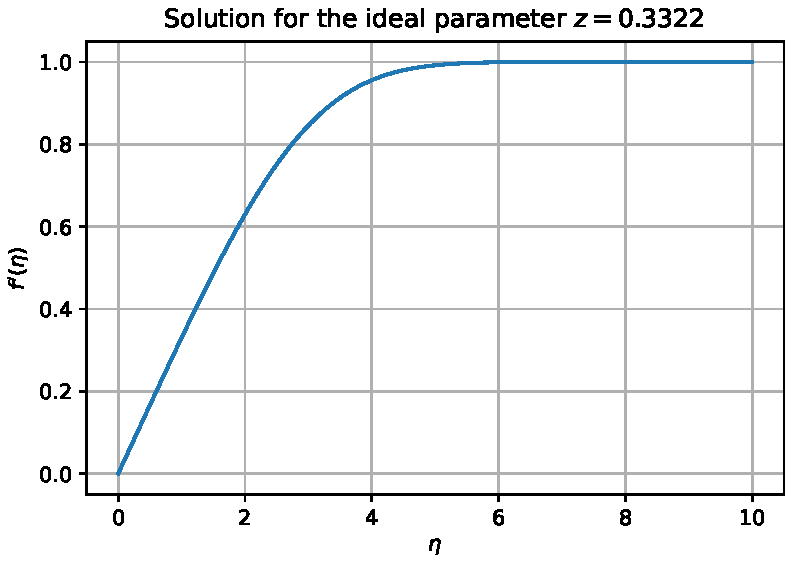
\includegraphics[width=0.75\textwidth]{plot_blasius_equation.pdf}
        \label{fig:blasius_solution}
    \end{figure}
    
    
    \question For this exercise we define the boundary-layer thickness $\delta$ such that $u = 0.9 V_{\infty}$. Using the stream function in the previous exercise calculate $\delta$ as a function of $x$. Interpret the result.
    
    \begin{solution}
        In weiser Voraussicht haben wir in der vorigen Aufgabe bereits das Argument der ersten Ableitung $f'$ zum Funktionswert $0.9$ bestimmt. Die Newtoniteration ergab den Wert $\eta \approx 3.39$. Wir wissen, dass 
        \begin{equation*}
            u = V_{\infty} f'(\eta) \overset{!}{=} V_{\infty} 0.9.
        \end{equation*}
        Da $\eta := y \sqrt{\frac{V_{\infty}}{\nu x}} = \delta \sqrt{\frac{V_{\infty}}{\nu x}} \approx 3.39 $, ergibt Umformen auf $\delta$
        \begin{equation*}
            \delta \approx \frac{3.39 x}{\sqrt{\operatorname{Re}_x}},
        \end{equation*}
        wobei $\operatorname{Re}_x = \frac{\rho_{\infty} V_{\infty} x}{\mu}$.
        
        {\color{red} TODO Interpret}
    \end{solution}
    
    
    \question We assume a boundary layer flow over a two-dimensional flat plate of length $L$. We assume that the velocity in the $x$-direction, denoted by $u(y)$, is independent of $x$. Show that for the skin friction drag $D_f$ (the force acting on the plate due to viscosity) we have
    \begin{equation*}
        D_f = \mu L \del_y u \vert_{y=0}.
    \end{equation*}
    Hint: If we consider only viscous effects, the force in the $x$-direction, $F_1$, acting on a fluid parcel $\Omega$ is given by
    \begin{equation*}
        F_1 = \int_\Omega \mu \Delta u \, d \mathbf{x}.
    \end{equation*}
    Choose $\Omega = [0, L] \times [0, \infty)$ and simplify the integral. Then invoke Newton's second law.
    
    \begin{solution}
        {\color{red} TODO}
    \end{solution}
    
    
    \question Linearize the Navier-Stokes equations
    \begin{align*}
        \del_t \rho + \nabla \cdot (\rho u) &= 0 \\
        \del_t \rho + (u \cdot \nabla) u + \frac{1}{\rho} \nabla p &= \frac{\mu}{\rho} \Delta u
    \end{align*}
    to obtain the damped wave equation
    \begin{equation*}
        \del_{tt} \rho_1 - \frac{\mu}{\rho_0} \Delta \del_t \rho_1 = RT \Delta \rho_1.
    \end{equation*}
    Show that if we assume $(\mu / \rho_0)^2 k^2 \ll RT$ the dispersion relations, in one-dimension, can be written as
    \begin{equation*}
        \omega(k) = \pm \sqrt{RT}k - i \frac{\mu}{2 \rho_0} k^2.
    \end{equation*}
    Derive the corresponding plane wave solutions and interpret your results.
    
    \begin{solution}
        {\color{red} TODO}
    \end{solution}
    
    
    \question We consider the toy model
    \begin{equation*}
        \del_t u(t,x) + \frac{1}{2} \del_x(u^2(t,x)) = \frac{1}{\text{Re}} \del_{xx} u(t,x) + \sin(2 \pi x), \qquad u(0,x) = 0.
    \end{equation*}
    A simple space discretization consists of introducing $u_i(t) = u(t, x_i)$, $x_i = ih$, $h = 1/n$ for $i = 0, \ldots, n - 1$ and using
    \begin{equation*}
        u_i'(t) = - \frac{u_i^2 - u_{i-1}^2}{2h} + \frac{1}{\text{Re}} \frac{u_{i+1} - 2u_i + u_{i-1}}{h^2} + \sin(2 \pi x_i).
    \end{equation*}
    We further set $u_{-1} = u_{n-1}$ and $u_n = u_0$. This is an ordinary differential equation which we can integrate using the explicit Euler method. In all simulations we use a (time) step size $\tau = 10^{-3}$ and $n = 100$. \newline
    Plot, on a double logarithmic scale, the absolute value of the the Fourier coeffcients corresponding to positive frequencies at time $t = 0.6$ for $\operatorname{Re} = 50$, $\operatorname{Re} = 200$, and $\operatorname{Re} = 800$.
    
    \begin{solution}
        {\color{red} TODO}
    \end{solution}
    
\end{questions}

\end{document}
